\documentclass[12pt,a4paper]{article}
%\usepackage{fontspec, xunicode, xltxtra}  
%\setmainfont{Hiragino Sans GB}  
\usepackage{xeCJK}
%\setCJKmainfont[BoldFont=STZhongsong, ItalicFont=STKaiti]{STSong}
%\setCJKsansfont[BoldFont=STHeiti]{STXihei}
%\setCJKmonofont{STFangsong}

%使用Xelatex编译

% 设置页面
%==================================================
\linespread{2} %行距
% \usepackage[top=1in,bottom=1in,left=1.25in,right=1.25in]{geometry}
% \headsep=2cm
% \textwidth=16cm \textheight=24.2cm
%==================================================

% 其它需要使用的宏包
%==================================================
\usepackage[colorlinks,linkcolor=blue,anchorcolor=red,citecolor=green,urlcolor=blue]{hyperref} 
\usepackage{tabularx}
\usepackage{authblk}         % 作者信息
\usepackage{algorithm}     % 算法排版
\usepackage{amsmath}     % 数学符号与公式
\usepackage{amsfonts}     % 数学符号与字体
\usepackage{graphics}
\usepackage{color}
\usepackage{fancyhdr}       % 设置页眉页脚
\usepackage{fancyvrb}       % 抄录环境
\usepackage{float}              % 管理浮动体
\usepackage{geometry}     % 定制页面格式
\usepackage{hyperref}       % 为PDF文档创建超链接
\usepackage{lineno}          % 生成行号
\usepackage{listings}        % 插入程序源代码
\usepackage{multicol}       % 多栏排版
%\usepackage{natbib}         % 管理文献引用
\usepackage{rotating}       % 旋转文字,图形,表格
\usepackage{subfigure}    % 排版子图形
\usepackage{titlesec}       % 改变章节标题格式
\usepackage{moresize}   % 更多字体大小
\usepackage{anysize}
\usepackage{indentfirst}  % 首段缩进
\usepackage{booktabs}   % 使用\multicolumn
\usepackage{multirow}    % 使用\multirow
\usepackage{graphicx} 
\usepackage{wrapfig}
\usepackage{xcolor}
\usepackage{titlesec}     % 改变标题样式
\usepackage{enumitem}

\renewcommand{\vec}[1]{\boldsymbol{#1}}
\newcommand{\me}{\mathrm{e}}
\newcommand{\mi}{\mathrm{i}}
\newcommand{\dif}{\mathrm{d}}
\newcommand{\tabincell}[2]{\begin{tabular}{@{}#1@{}}#2\end{tabular}}

\def\kpc{{\rm kpc}}
\def\km{{\rm km}}
\def\cm{{\rm cm}}
\def\TeV{{\rm TeV}}
\def\GeV{{\rm GeV}}
\def\MeV{{\rm MeV}}
\def\GV{{\rm GV}}
\def\MV{{\rm MV}}
\def\yr{{\rm yr}}
\def\s{{\rm s}}
\def\ns{{\rm ns}}
\def\GHz{{\rm GHz}}
\def\muGs{{\rm \mu Gs}}
\def\arcsec{{\rm arcsec}}
\def\K{{\rm K}}
\def\microK{\mu{\rm K}}
\def\sr{{\rm sr}}
\newcolumntype{p}{D{,}{\pm}{-1}}

\renewcommand{\figurename}{Fig.}
\renewcommand{\tablename}{Tab.}

\renewcommand{\arraystretch}{1.5}

\setlength{\parindent}{0pt}  %取消每段开头的空格

\title{宇宙热历史}
\author{}
\date{\today}
\begin{document}

\maketitle

\cite{perkins2008particle} For the radius of the universe we have simply quoted the \textcolor{red}{Hubble length $c t_0$} where $t_0 = 14$ Gyr is the age of the universe. On account of the Hubble expansion, the actual radius of the visible universe --- the distance to the optical horizon --- is larger than the Hubble length, and according to our present ideas, about a factor $3.3$ times larger. 

The (negative) gravitational potential energy $GM^2/R$ and the mass energy $M c^2$ of the universe are comparable at $\sim 10^{70}$ J, so that the total energy could be quite small. The measured value of the curvature parameter on very large scales is consistent with it, and the total energy, being exactly zero.

The distance is estimated from the apparent brightness or luminosity, and is therefore called the luminosity distance $D_L$. It is determined from the (supposedly known) intrinsic luminosity $L$ or total power radiated by the source (star or galaxy), and the measured energy flux $F$ at the Earth
\begin{equation}
F = \dfrac{L}{4\pi D_L^2} ~.
\end{equation}

The astronomers use a \textcolor{orange}{logarithmic scale of luminosity}, called \textcolor{red}{magnitude}, running (perversely) from small values of magnitude for the brightest stars to large values for the faintest. The defining relation between the \textcolor{red}{apparent magnitude} $m(z)$ at redshift $z$, the so-called \textcolor{red}{absolute magnitude} $M$ (equal to the value that $m$ would have at $D_L = 10$ pc) and the distance $D_L$ in Mpc, is given by the \textcolor{red}{distance modulus}
\begin{equation}
m(z) - M = 5 \log_{10} D_L(z) +25 ~.
\end{equation}

Once the universe had cooled to a temperature $kT < 100$ MeV, or after a time $t > 10^{-4}$ s, essentially all the hadrons, with the sole exception of neutrons and protons and their antiparticles, would have disappeared by decay. The nucleons and antinucleons would have been present
in equal numbers and have nearly, but not quite completely, annihilated to radiation. Once the temperature had fallen below $kT = 20$ MeV, a tiny residue of about one billionth of the original numbers of protons and neutrons must have survived to form the stuff of the material universe we inhabit today. The \textcolor{orange}{relative numbers of these surviving protons and neutrons} would have been determined by the \textcolor{orange}{weak reactions}
\begin{align}
\nu_{e} +n \leftrightarrow {\rm e}^- + p ~, \\
\bar{\nu}_e +p \leftrightarrow {\rm e}^+ + n ~, \\
n \leftrightarrow p +{\rm e}^- +\bar{\nu}_e ~.
\end{align}


\cite{ryden2016introduction} The cosmic microwave background tells us a great deal about the state of the universe at the time of last scattering ($t_{\rm ls} \approx 0.37$ Myr). The opacity of the early universe prevents us from directly seeing what the universe was like at $t < t_{\rm ls}$. when radiation is strongly dominant over matter, at scale factors $a \ll a_{\rm rm} \approx 2.9 \times 10^{-4}$, or times $t \ll t_{\rm rm} \approx 50 000$ yr, the expansion of the universe has the simple power-law form $a(t) \propto t^{1/2}$. The temperature of the blackbody photons in the early universe, which decreases as $T \propto a^{-1}$ as the universe expands, is given by the convenient relation
\begin{equation}
T(t) \approx 10^{10}~ {\rm K} \left(\dfrac{t}{1~ \rm s} \right)^{-1/2} ~,
\end{equation}
or
\begin{equation}
k T(t) \approx 1~ {\rm MeV} \left(\dfrac{t}{1~ \rm s} \right)^{-1/2} ~.
\end{equation}
The mean energy per photon was
\begin{equation}
E_{\rm mean}(t) \approx 2.7 kT(t) \approx 3 {\rm MeV} \left(\dfrac{t}{1~ \rm s} \right)^{-1/2} ~.
\end{equation}

\cite{2012宇宙大尺度结构的形成} 用温度$T$描述宇宙演化过程,$kT$表示粒子热运动能量的典型值;

在辐射为主阶段它与宇宙年龄$t$($s$为单位)的关系
\begin{equation}
\frac{T}{\text{MeV}} \approx \frac{T}{10^{10} \text{K}} \approx \frac{1}{\sqrt{t}}
\end{equation}
随着宇宙(绝热)膨胀,温度及能量密度都逐渐降低



\cite{cheng2005relativity}

\section{Olbers' paradox} 
\cite{perkins2008particle} Supposed the universe to be unlimited in extent and filled uniformly with sources of light (stars). The light flux reaching us from a star at distance $r$ varies as $r^{-2}$, while the number of stars in the spherical shell $r \rightarrow r +\dif r$ varies as $r^2 \dif r$. Hence the total light flux will increase as $r$(max), which is infinite in the model.

The observable universe is not infinite but has a finite age, and began at a time $t_0$ in the past with the Big Bang which started off the Hubble expansion. This means that light can only reach us from a maximum horizon distance $c t_0$, and the flux must be finite.

The light sources (stars) are finite in size, so that nearby sources will block out light from more distant sources. Their light is absorbed exponentially with distance by the intervening stars and dust.

Stars only emit light for a finite time $t$, and the flux from the most distant stars will be reduced by a factor $t/t_0$.

The expansion of the universe results in an attenuation at large enough redshifts of light of any particular frequency.

\cite{2015eaci.book.....S} Let $n_\ast$ be the mean number density of stars, constant in space and time according to the assumptions, and let $R_\ast$ be their mean radius. A spherical shell of radius $r$ and thickness $\dif r$ around us contains $n_\ast \dif V = 4\pi r^2  \dif r n_\ast$ stars. Each of these stars subtends a solid angle of $\pi R_\ast^2/ r^2$ on our sky, the stars in the shell cover a total solid angle of
\begin{equation}
\dif \omega = 4\pi r^2 \dif r n_\ast \dfrac{R_\ast^2 \pi}{r^2} = 4\pi^2 n_\ast R_\ast^2 \dif r ~.
\end{equation}
This solid angle is independent of the radius $r$ of the spherical shell because the solid angle covered by a single star $\propto r^{-2}$ just compensates the volume of the shell $\propto r^2$. To compute the total solid angle of all stars in a static Euclidean universe, integrate over all distances $r$, but the integral
\begin{equation}
\omega = \int_0^\infty \dif r \dfrac{\dif \omega}{\dif r} = 4\pi^2 n_\ast R_\ast^2 \int_0^\infty \dif r ~,
\end{equation}
diverges. Formally, this means that the stars cover an infinite solid angle, which of course makes no sense physically. The reason for this divergence is that we disregarded the effect of overlapping stellar disks on the sphere. However, these considerations demonstrate that the sky would be completely filled with stellar disks, i.e., from any direction, along any line-of-sight, light from a stellar surface would reach us. Since the specific intensity $I_\nu$ is independent of distance --- the surface brightness of the Sun as observed from Earth is the same as seen by an observer who is much closer to the Solar surface --- the sky would have a temperature of $\sim 10^4$ K.





\section{CMB radiation}
\cite{perkins2008particle} Recent data show very precise agreement with the spectrum expected from a black body at a temperature of $2.725 \pm 0.001$ K; indeed, the cosmic microwave spectrum is the black body spectrum par excellence. It proves among other things that at the time the radiation last interacted significantly with matter, it was in thermal equilibrium with it. In fact, the CMB observed today originated when matter and radiation decoupled as the universe expanded and cooled, some $380,000$ years after the Big Bang.

Assuming that matter has been conserved, the matter density of the universe can be expected to vary as $\rho_m \propto R^{-3}$. On the other hand, the density of radiation, assuming it to be in thermal equilibrium, will vary with temperature as $\rho_r \propto T^4$ (Stefan's Law). Since there is no absolute scale of distance, the wavelength of the radiation on the truly cosmic scale associated with the Hubble expansion can only be proportional to the expansion factor $R$. Thus the frequency $\nu = c/\lambda$ and the mean energy per photon will both be proportional to $R^{-1}$. While the number of photons varies as $1/R^3$, the energy density of the radiation will vary as $1/R^4$. 

While the matter density of the universe dominates over radiation today, in the olden days and at low values of R, radiation must have been dominant. 
\begin{equation}
\dot{R}^2 = \left( \dfrac{8\pi G}{3} \right) \rho_r R^2 ~.
\end{equation}
Since $\rho_r \propto R^{-4}$,
\begin{equation}
\dfrac{\dot{\rho}_r}{\rho_r} = - \dfrac{4\dot{R}}{R} = -4 \left( \dfrac{8\pi G \rho_r }{3} \right)^{1/2} ~, 
\end{equation}
which on integration gives for the energy density
\begin{equation}
\rho_r c^2 = \left( \dfrac{3c^2 /32\pi G}{t^2} \right) ~.
\end{equation}
For a photon gas in thermal equilibrium
\begin{equation}
\rho_r c^2 = \dfrac{4\sigma T^4}{c} = \pi^4 (kT)^4 \left( \dfrac{g_\gamma/2}{15\pi^2 \hbar^3 c^3} \right)~,
\end{equation}
$g_\gamma = 2$ is the number of spin substates of the photon. A relation between the temperature of the radiation
and the time of expansion
\begin{equation}
kT = \dfrac{\left[(45\hbar^3 c^5/16\pi^3 G g_\gamma)^{1/4}\right]}{t^{1/2}} = 1.307~ \dfrac{{\rm MeV}}{t^{1/2}} ~,
\label{eq:T_t}
\end{equation}
where $t$ is in seconds. The corresponding value of the temperature itself is
\begin{equation}
T = 1.52\times 10^{10} \dfrac{K}{t^{1/2}} ~.
\end{equation}
Since $T$ falls as $1/R$, $R$ increases as $t^{1/2}$ while the temperature falls as $1/t^{1/2}$. Hence, the universe started out as a hot Big Bang.

From Eq. (\ref{eq:T_t}), we may roughly \textcolor{green}{estimate the energy of the radiation today}, that is for $t_0 \sim 14$ Gyr $\sim 10^{18}$ s. 

Observation of microwave molecular absorption bands in distant gas clouds has made it possible to estimate the temperature of the background radiation at earlier times, when the wavelength would have been reduced, and the temperature increased, by theredshiftfactor $(1+z)$. This dependence on redshift has been experimentally verified up to values of $z \approx 3$. 

The temperature of the microwave radiation shows a small anisotropy, of order $10^{-3}$, attributed to the \textcolor{blue}{`peculiar velocity' $v = 370$ km s$^{-1}$ of the Solar System (towards the Virgo cluster) with respect to the (isotropic) radiation}. It is given by the Doppler formula 
\begin{equation}
\color{yellow} T(\theta) = T(0) \left[1 + \left(\dfrac{v}{c} \right) \cos \theta \right] ~,
\end{equation}
where $\theta$ is the direction of observation with respect to the velocity $v$.

The microwave radiation, previously in equilibrium with atomic and ionized hydrogen, decoupled from baryonic matter
at $z \sim 1100$, when the universe was about $400,000$ years old. That would have been the epoch of `last scattering', if the interstellar gas (mostly hydrogen and helium) remained \textcolor{yellow}{unionized}. However, it appears that when $z$ fell below about $12$ (the end of the so-called \textcolor{red}{dark ages}), the first stars had formed and commenced re-ionization of the intergalactic medium, by the ultraviolet radiation they emitted. Thus the microwave radiation, on its \textcolor{blue}{passage through the interstellar medium to the observer}, would then undergo \textcolor{blue}{Thomson scattering from electrons} in the plasma.

\cite{cheng2005relativity} For the radiation component of the universe, we can neglect particle masses and chemical potentials\footnote{Except that for photons, there is no strong theoretical ground to set the chemical potential $\mu$ to zero. Yet, since there is nothing that requires a sizable $\mu$, we shall for simplicity
set $|\mu| \ll k_{\rm B}T$.} compared to $k_{\rm B}T$, where $k_{\rm B}$ is the Boltzmann constant. The number distributions with respect to the energy $E$ of the radiation system composed of bosons (for the minus sign) and fermions (for the positive sign) are, respectively,
\begin{equation}
\dif n = \dfrac{4\pi g}{h^3 c^3} \dfrac{E^2 \dif E}{e^{E/k_{\rm B}T} \pm 1} ~,
\end{equation}
with $h$ the Planck constant, and $g$ the number of spin states of the particles making up the radiation; for photons and electrons, we have $g(\gamma) = 2$ and $g(e) = 2$, respectively,\footnote{Particles, with mass and spin $s$, have $2s +1$ spin states (e.g. spin $1/2$ electrons have two spin states), but massless spin particles (e.g. spin $1$ photons or spin $2$ gravitons) have only two spin states.}  neutrinos have $g(\nu) = 1$ because only the left-handed spin states participate in interactions. The number density is $n = \int \dif n \sim T^3$, 
\begin{equation}
n_b = \dfrac{4}{3} n_f = 2.404 \dfrac{g}{2\pi^2} \left(\dfrac{k_{\rm B}T}{hc} \right)^3 ~,
\end{equation}
for the respective boson and fermion systems. We can derive the thermodynamic relation (the Stefan–Boltzmann law) between radiation energy density $(u)$ and its temperature by performing the integration of $u = \int E \dif n \sim T^4$:
\begin{equation}
\rho_R c^2 \equiv u_R = \dfrac{g^\ast}{2} a_{\rm SB} T^4 ~,
\end{equation}
where $a_{\rm SB}$ is the Stefan–Boltzmann constant. We have summed over the energy contribution by all the constituent radiation particles so that $g^\ast$ is the ``effective number" of spin states of the particles making up the radiation:
\begin{equation}
g^\ast = \sum_i (g_b)_i +\dfrac{7}{8} \sum_i (g_f)_i ~,
\end{equation}
where $(g_b)_i$ and $(g_f)_i$ are the spin factors of the $i$th species of boson and fermion radiation particles, respectively. The $\dfrac{7}{8}$ factor reflects the different integral values for the fermion distribution, with a plus sign, vs. the minus sign for the boson case.

\section{Particles and radiations in the early universe}
\cite{perkins2008particle} The relation (\ref{eq:T_t}) for the temperature of the early universe as a function of time applies for radiation consisting of photons (with $g_\gamma = 2$). Relativistic fermions, that is, quarks and leptons, assuming that they are stable enough, would also contribute to the energy density. For a fermion gas, the FD distribution for the number density analogous to (\ref) is
\begin{equation}
N(p) \dif p = \dfrac{p^2 \dif p}{\pi^2 \hbar^3 \left[1 +\exp (E/kT) \right]} \left( \dfrac{g_f}{2} \right) ~,
\end{equation}
where $E^2 = p^2 c^2 + m^2 c^4$, $m$ is the fermion mass and $g_f$ is the number of spin substates. In the relativistic limit, $kT \gg mc^2$ and $E = pc$, the total energy density is given by
\begin{equation}
\rho_f c^2 = \left( \dfrac{7}{8} \right) \pi^4 (kT)^4 \dfrac{g_f/2}{15 \pi^2 \hbar^3 c^3}  ~ .
\end{equation}
For a mixture of extreme relativistic bosons $b$ and fermions $f$, the energy density is found by replacing $g_\gamma$ by a factor \textcolor{red}{$g^\ast$} where
\begin{equation}
\color{red} g^\ast = \sum g_b +\left( \dfrac{7}{8} \right) \sum g_f ~,
\end{equation}
and the summation is over all types of relativistic particles and antiparticles which contribute to the energy density of radiation in the early universe.

At very early times when the temperature was high enough for their creation, all types of elementary quarks, leptons, and bosons, plus their antiparticles, would have been present in the primordial `soup' in which the various components would have been in thermal equilibrium. On the basis of the fundamental particles we know today, the number of degrees of freedom (charge, spin, and colour substates) of the fermions would be $90$, and that of the gauge bosons $28$. The bosons include the massless photon of spin $1$, occurring in $2$ spin states since, according to relativistic invariance, a massless particle of spin $J$ can have only two substates, $J_z = \pm J$ ; the massless gluon also of spin $1$, $2$ spin substates, and $8$ substates of colour; the massive bosons $W^+$, $W^-$, and $Z_0$, again of spin $1$ but since they are massive, contribute $2J +1 = 3$ spin substates each; and finally the Higgs scalar spin $0$ boson of the electroweak theory, bringing the total to $28$. The fermions include the quarks, occurring in $6$ flavour states, $3$ colour, and $2$ spin substates, plus their antiparticles, totalling $72$ states altogether; the charged leptons in $3$ flavour and $2$ spin substates, plus their antiparticles, that is a total of $12$ states; and finally the neutral leptons (neutrinos) in $3$ flavours but only one spin substate each. Including antiparticles the neutrinos contribute $6$ degrees of freedom, making $90$ fermion and antifermion states in total. If
supersymmetry is valid, the number of states will be approximately doubled. For values of $kT$ very much larger than any of the particle masses, then inserting $g_b = 28$ and $g_f = 90$, the value of \textcolor{red}{$g^\ast = 106.75$}, as shown inf Fig. \ref{fig:geff}. 

As the expansion proceeded and the temperature fell, the most massive particles, such as the \textcolor{blue}{top quark} and the \textcolor{blue}{$W$} and \textcolor{blue}{$Z$ bosons} would have been \textcolor{blue}{rapidly lost by decay} (in \textcolor{blue}{less than $10^{-23}$ s}) and not replenished once $kT \ll Mc^2$ where $M$ is the particle mass. After \textcolor{blue}{$kT$ fell below the strong quantum chromodynamics (QCD) scale parameter $\sim 200$ MeV}, the remaining quarks, antiquarks, and gluons would no longer exist as separate components of a plasma but as quark bound states, \textcolor{blue}{forming the lighter hadrons such as pions and nucleons}. However, all hadrons except protons and neutrons would be too short-lived to exist beyond the first few nanoseconds. Similarly, the \textcolor{blue}{charged muon} and \textcolor{blue}{tauon} leptons would \textcolor{blue}{decay within the first microsecond or so}. Once $kT$ had \textcolor{blue}{fallen below about $20$ MeV}, that is \textcolor{blue}{after the first few milliseconds}, \textcolor{blue}{most of the nucleons and antinucleons would also have annihilated to radiation}. The \textcolor{blue}{surviving number of nucleons} amounts to only about \textcolor{blue}{one billionth of the number of photons}. This would leave, apart from the photons, the electrons $e^-$ and the $\nu_e$, $\nu_\mu$, and $\nu_\tau$ neutrinos, plus their antiparticles, giving \textcolor{blue}{$\sum g_f = 4 + 2 + 2 +2$} (recalling \textcolor{blue}{two spin states each for electrons and positrons}, but only \textcolor{blue}{one for the neutrinos or antineutrinos}). With $g_b = 2$ for the photon this results in a value \textcolor{blue}{$g^\ast = 43/4$}. The effect is to multiply the expression for $kT$ on the extreme right-hand side of (\ref{eq:T_t}) by a factor \textcolor{blue}{$(g^\ast/2)^{-1/4}$}, which has the value \textcolor{blue}{$0.66$}. Note that this result applies for values of $kT$ between about $20$ MeV and $5$ MeV, as is shown in Fig. \ref{fig:geff}. 


%===========================================================================================================================
\begin{figure}
\centering
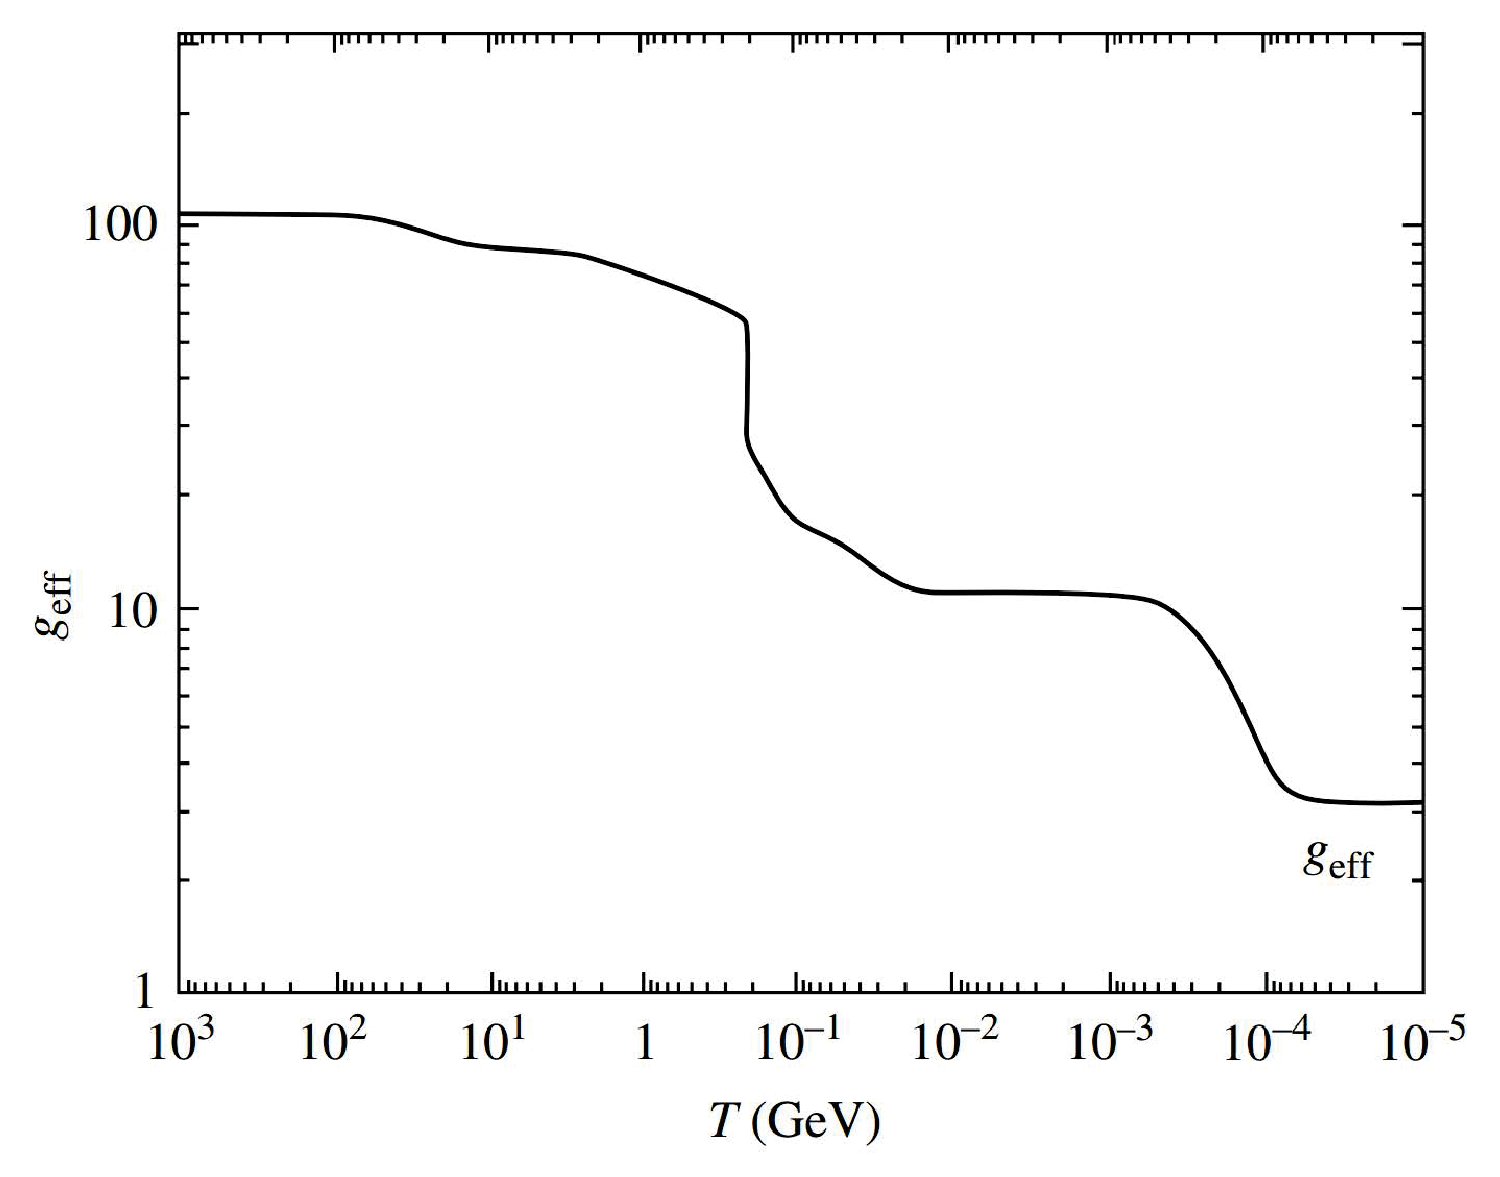
\includegraphics[height=9.cm,angle=0]{geff.eps}
\caption{} 
\label{fig:geff}
\end{figure}
%===========================================================================================================================

The Hubble parameter $H(t)$ in terms of the temperature $T$ in the radiation-dominated era of the early universe. Since in this era, $\rho \propto R^{-4}$,
\begin{equation}
H(t) = \dfrac{\dot{R}}{R} = - \dfrac{\dot{\rho}}{4\rho}  = \dfrac{1}{2t} ~,
\end{equation}
and
\begin{align}
\nonumber H(t) &= \left[\dfrac{4g^\ast \pi^3 G}{45 \hbar^3 c^5} \right] (kT)^2 \\
\nonumber &= \dfrac{(4 \pi^3 g^\ast \pi^3 /45)^{1/2}}{M_{\rm PL} \hbar c^2} (kT)^2 \\
&= 1.66 g^{\ast 1/2} \dfrac{(kT)^2}{M_{\rm PL} \hbar c^2} ~,
\end{align}
where $G = \hbar c/M_{\rm PL}^2$.

\section{Photon and neutrino densities}


\section{普朗克时期}
$T \sim 10^{32}$ K,$kT \sim E_{pl} \simeq 10^{19}$ GeV,$t \sim 10^{-43}$ s



\section{宇宙暴涨}
$T \sim 10^{26}$ K,$kT \sim 10^{15}$ GeV,$t \sim 10^{-33}$ s


\section{强子时期}


\section{轻子时期}

\section{轻元素核合成}
$T \sim 10^{9}$ K


\section{复合时期}
$T \approx 4000 - 3000$ K



\section{星系形成}

观测结果表明:许多星系和类星体在$1<z<6$期间形成,在$6<z<10$之间星系或类星体的数目非常稀少,而$z>10$的天体目前还没有观测到


$T \leq 1000$ K

Dark Ages:$10 < z < 1000$









%%%%%%%%%%%%%%%%%%%%%%%%%%%%%%%%%%%%%%%%%%%%%%%%%%%%%%%%%%%%%%%%%%%%%%
\bibliographystyle{unsrt_update}
\bibliography{ref}
%%%%%%%%%%%%%%%%%%%%%%%%%%%%%%%%%%%%%%%%%%%%%%%%%%%%%%%%%%%%%%%%%%%%%%


\end{document}